\section{Can the degradation be detected early?}
\label{sec:monitoring}

A deployed information system does not observe accuracy. We therefore asked whether
the framework of Section~\ref{sec:framework} would have warned, at three
levels: the direction of the quality metrics, the alarms of calibrated
single-stream detectors, and the power such detectors can have at all.
Table~\ref{tab:warningsummary} summarises the tests; none yielded robust,
model-general early warning.

\begin{table}[!htbp]
\centering
\caption{Summary of the early-warning tests (labels as in
Section~\ref{sec:framework}).}
\label{tab:warningsummary}
\footnotesize
\setlength{\tabcolsep}{4pt}
\begin{tabular}{@{}>{\raggedright\arraybackslash}p{0.20\linewidth}
>{\raggedright\arraybackslash}p{0.24\linewidth}
>{\raggedright\arraybackslash}p{0.15\linewidth}
>{\raggedright\arraybackslash}p{0.33\linewidth}@{}}
\toprule
Setting & Signal & Label & Outcome\\
\midrule
Study 1, pre-final turns & CS, LS, SS vs.\ final failure & confirmatory &
no association; all Holm $p=1.0$\\
Study 1 & CRL (paired readiness) & confirmatory, auxiliary & modest AUROC
\crlAuroc{}; nothing beyond the last readiness gap (post hoc)\\
Study 1 replay & five detectors on CQ, CS, RS, LS, SS & post hoc &
detection $\le0.067$ under family-wise control; no candidate\\
Study 2, history arm & six metrics, three strategies & confirmatory &
CQ nulls also collapse, so thresholds cannot be calibrated; other metrics
$\le0.11$\\
Study 2, GPT-4o-mini control & CQ, LS, ES detectors and a threshold rule &
exploratory & CUSUM \ctrlScreenDetect{}; LS leads not separable from null
alarms\\
Study 2, Llama/Gemma control & unchanged rules & frozen validation &
screen failed in both models\\
Study 2, six-dialogue aggregates & CQ CUSUM & exploratory & all drift
scenarios detected; one stationary alarm (Gemma)\\
\bottomrule
\end{tabular}
\end{table}

\subsection{Quality metrics do not fall with accuracy}

A post-hoc replay of Study~1 suggests why the pre-final metrics gave no
detectable warning (Figure~\ref{fig:silent}b). When completed sessions were streamed with
a switch from fresh prefix to dialogue history, coherence and stability
\emph{rose} while accuracy fell: in the sudden scenario at $W=20$, the median
Cliff's $\delta$ \citep{cliff1993dominance} between the last pre-change and the
last stream window was \replaySsDeltaGpt{} for SS in GPT-4o-mini,
\replaySsDeltaLlama{} in Llama-4 Scout, and \replayLsDeltaGpt{} for LS in
GPT-4o-mini. Study~2 shows the same pattern over 100 turns
(Figure~\ref{fig:silent}a, descriptive). For GPT-4o-mini under dialogue
history, accuracy fell from \silentCQEarly{} (turns 1--5) to \silentCQLate{}
(turns 81--100), while stability rose from \silentSSEarly{} to \silentSSLate{}
and coherence moved only from \silentLSEarly{} to \silentLSLate{}. Consistency
declined from \silentCSEarly{} to \silentCSLate{}, but slowly, long after most
accuracy was lost, and it even rose over turns 6--15 as accuracy halved. As the
model fails, its replies become more alike and stay locally coherent. A
monitor that alarms on decreases cannot detect this, and a two-sided monitor
would detect a change whose sign says nothing reliable about correctness.

\begin{figure}[!htbp]
\centering
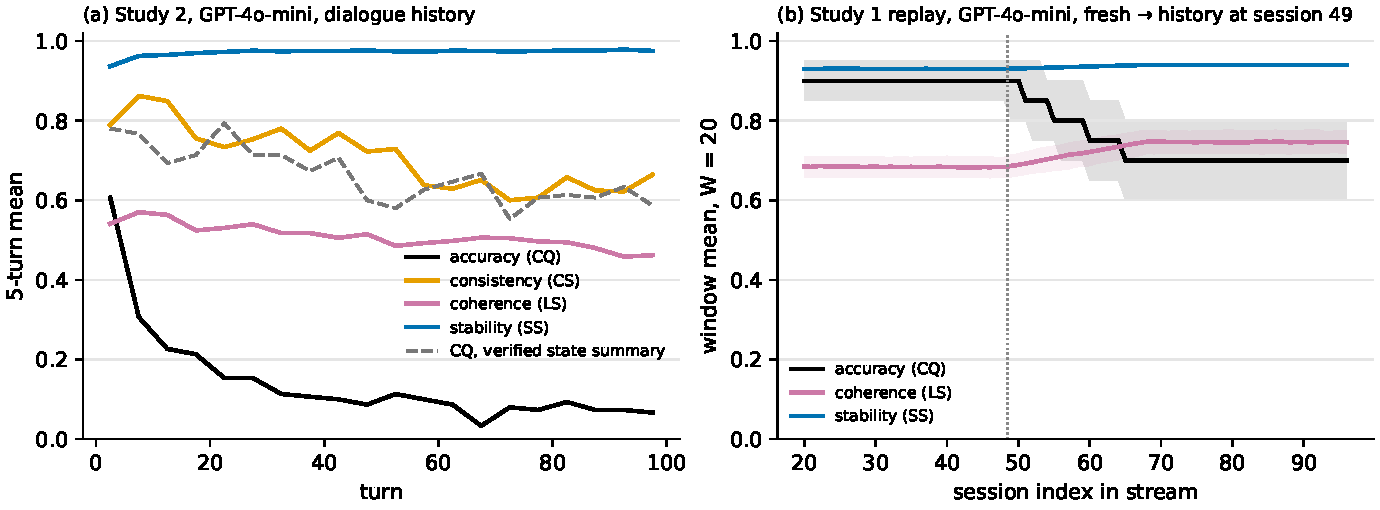
\includegraphics[width=\linewidth]{silent_metrics.pdf}
\caption{Quality metrics do not track accuracy. (a) Study 2, GPT-4o-mini,
dialogue history, 5-turn means over 30 dialogues (descriptive); dashed:
accuracy under the verified state summary; CS is supported by
\silentCsSupport{} of 3,000 turns. (b) Post-hoc replay of Study 1: median and
10--90\% band over 1,000 orderings of window means ($W=20$) when the regime
switches from fresh prefix to dialogue history at session 49.}
\label{fig:silent}
\end{figure}

\subsection{Calibrated single-stream detectors}

In the Study~1 replay (post hoc), with thresholds calibrated on 2,000
permutation nulls at family-wise $\alpha=0.05$ and validated on 2,000 disjoint
nulls, the best detection rate of any configuration was 0.067 (Mistral-7B, CQ,
sudden switch, median delay about 44 sessions); no metric qualified
(supplementary Table~S3). In this replay the stream items
are completed sessions, not turns, and a detection is any first alarm after
the switch, so the 33-turn window of Definition~2 does not apply; the delay is
counted in sessions.

In the Study~2 dialogue arm (confirmatory), the stationary dialogues that should
serve as nulls collapsed themselves. For CQ no grid value met the 5\% null
false-alarm target in most configurations, and the other metrics detected at
most 0.11 of drifts within 33 turns (supplementary
Table~S9). This is the core difficulty of monitoring under
accumulated history: the decline starts at turn~1, before any reference period,
in exactly the streams that define normal behaviour.

The verified-state arm removes this background collapse and leaves only the
scheduled task drift, so it is the cleanest test of the detectors. On
GPT-4o-mini (exploratory), CUSUM on the window mean of CQ detected
\ctrlScreenDetect{} drift dialogues within 33 turns at $W=20$, partly because
the detectors ignore their first 20 window values, which places the earliest
alarm near turn 40, after the first change at 34. A simpler rule, a window mean
below $\mu_0-2\sigma_0/\sqrt{W}$ for three turns with $\mu_0,\sigma_0$ from turns
1--30, flagged accuracy in \earlyCqSignal{} drift but also \earlyCqNull{}
stationary dialogues. LS signalled in \earlyLsSignal{} drift dialogues,
\earlyLsBefore{} of them before accuracy, but also in \earlyLsNull{} stationary
ones. Applied unchanged to the unseen Llama-3 70B and Gemma 3 12B control arms
as a frozen validation, CUSUM detected \valLlamaDetect{} and \valGemmaDetect{}
drift dialogues (median delays \valLlamaDelay{} and \valGemmaDelay{} turns),
and the LS rule signalled in \valLlamaLsSignal{} and \valGemmaLsSignal{} drift
dialogues but also in \valLlamaLsNull{} and \valGemmaLsNull{} stationary ones.
Neither rule passed the frozen screen in either model.

Because the frozen monitor cannot alarm before turn 40, part of this failure
could reflect the monitor rather than the signals. A post-hoc audit
(supplementary Section~S6) removed the floor with a CUSUM on raw values
standardised against turns 1--30. On synthetic streams it caught a precursor
injected at turn 31 by turn 33 in 45\% of streams for a shift of 0.3 and in
nearly all for 0.5, where the frozen path caught none. On the control arms,
with thresholds set on GPT-4o-mini and transferred unchanged, the CQ detector
alarmed in 0.25 and 0.17 of the stationary Llama and Gemma dialogues, and LS
or ES alarmed before CQ in at most 3 of 5 dialogues in which both alarmed
(supplementary Table~S19). No non-CQ signal combined an early alarm, a
controlled false-alarm rate and transfer across models, so the negative result
does not rest on the turn-40 floor.

\subsection{Why single streams are underpowered}

These failures follow from the information in one 100-turn stream. A simple
bound shows the scale of the problem. Consider the accuracy window mean
(\ref{eq:windowmean}) pooled over $m$ dialogues that are at the same turn, so
that it averages $n=mW$ binary outcomes.

\begin{proposition}[Smallest detectable drop]
\label{prop:mindrop}
Let the $n=mW$ outcomes in the window be independent Bernoulli variables with
success probability $p_0$ before a change and $p_1=p_0-\delta$ after it, and
write $\sigma_i^2=p_i(1-p_i)$. Consider a one-sided test that alarms when the
window mean falls below a threshold set so that its false-alarm probability
under $p_0$ is $\alpha$. Under the normal approximation, the test detects the
drop with probability at least $\beta$ only if
\begin{equation}
  \delta \;\ge\; \frac{z_{1-\alpha}\,\sigma_0 + z_{\beta}\,\sigma_1}{\sqrt{mW}},
  \label{eq:mindrop}
\end{equation}
where $z_q$ is the $q$-quantile of the standard normal distribution.
\end{proposition}

\begin{pf}
Under $p_i$ the window mean is approximately normal with mean $p_i$ and
standard deviation $\sigma_i/\sqrt{n}$. A false-alarm probability $\alpha$
requires the threshold $k=p_0-z_{1-\alpha}\sigma_0/\sqrt{n}$. Under $p_1$ the
detection probability is $\Phi\!\left((k-p_1)\sqrt{n}/\sigma_1\right)$, which is
at least $\beta$ exactly when $(k-p_1)\sqrt{n}\ge z_\beta\sigma_1$. Substituting
$k$ and $p_0-p_1=\delta$ gives (\ref{eq:mindrop}).
\end{pf}

With $p_0=0.8$, $W=20$, $\alpha=0.05$ and $\beta=0.8$, the bound is about 0.24
for one dialogue, 0.10 for six and 0.05 for 18. A monitor looks at many turns,
so its per-look level must be smaller: splitting $\alpha$ over the 67 looks
from turn 34 to turn 100 raises the bound to 0.38, 0.15 and 0.09. Positive
dependence between successive turns lowers the effective $n$ and raises it
further. The proposition covers only a threshold on the window mean, not
CUSUM or the other detectors, so it explains the scale and the $1/\sqrt{m}$
gain from aggregation rather than predicting their exact power.

To measure the power of the detectors actually used, we simulated per-turn correctness streams with pre-change accuracy 0.80 and a drop
$\delta$ at turn 34 or 51, aggregating $m$ independent dialogues per turn, with
the unchanged detectors, thresholds from 12 null streams at a 5\% false-alarm
target, and 300 drift streams per cell (Figure~\ref{fig:power}). A single
stream reached 80\% detection within 33 turns only for drops of about 0.5,
whereas the task drifts in our data were 0.1--0.3. Aggregating six dialogues
per turn lowered the detectable drop to 0.2, and 18 dialogues to 0.1; results
were similar for other windows and calibration sets (supplementary
Table~S14). Applied exploratorily to the control arms, a
CQ CUSUM on six-dialogue scenario aggregates detected all three drift
scenarios in both validation models (\valLlamaAggDetect{} and
\valGemmaAggDetect{}), with no alarm in the Llama stationary aggregates and one
in the two Gemma ones (\valLlamaAggNull{}, \valGemmaAggNull{}). Aggregation
across sessions is thus promising, but too few aggregates and the Gemma false
alarm preclude a confirmatory claim. Small null sets also limit what a clean
result can show. With no alarm in $n$ null streams, the exact one-sided 95\%
upper bound on the false-alarm rate is $1-0.05^{1/n}$: 0.78 for two aggregates
and 0.22 for 12 dialogues. Our thresholds therefore meet a 5\% target on the
calibration nulls, but the true false-alarm rate is verified only within these
bounds.

\begin{figure}[!htbp]
\centering
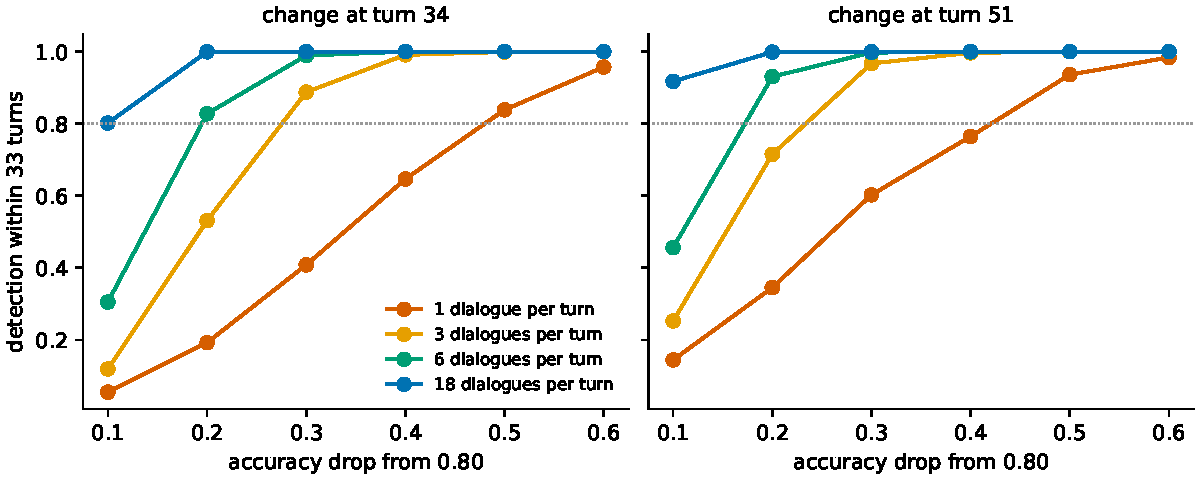
\includegraphics[width=\linewidth]{detector_power.pdf}
\caption{Simulated detection within 33 turns versus the accuracy drop from 0.80
and the number of dialogues aggregated per turn ($W=20$, thresholds from 12
null streams, 5\% false-alarm target). Left: change at turn 34; right: at
turn 51. Dotted line: 80\% detection.}
\label{fig:power}
\end{figure}

\subsection{A baseline that could not fire}

Our generic ADWIN baseline never alarmed, because our implementation omitted
the variance term of the cut bound of \citet{bifet2007learning}; without it, no
difference of means in at most 100 values in $[0,1]$ can exceed the bound.
Re-running every affected analysis with a corrected ADWIN and with CUSUM, as a
labelled sensitivity analysis, changed no conclusion: the corrected analyses
also produced no early-warning candidate for consistency or stability. Even
corrected ADWIN
needed drops of about 0.6 on 100-turn streams (supplementary
Table~S15). A generic baseline is a meaningful comparator only
once it has been shown to fire on streams of the intended length.
